	\subsection{UC 6 - Gestione view}

		\begin{figure}[H]
			\centering
			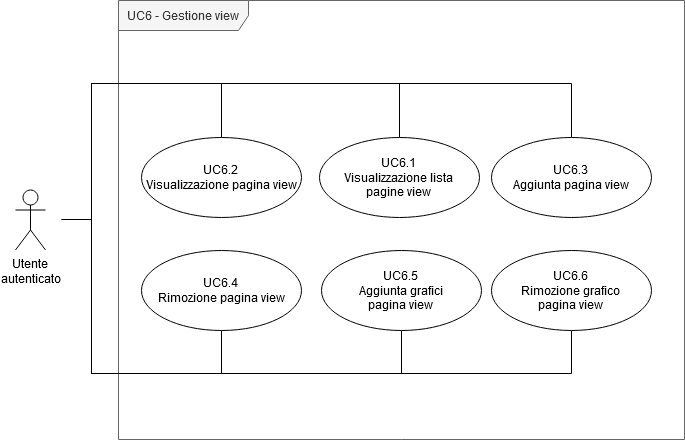
\includegraphics[scale=0.60]{res/images/uc6}
			\caption{Diagramma che riassume la gestione delle view con cui può interagire l'utente nella web app.}
		\end{figure}

		\begin{itemize}
			\item \textbf{Attori Primari}: Utente autenticato.
			\item \textbf{Descrizione}: L'utente può gestire le proprie pagine \glock{view}, attraverso cui può andare a visualizzare grafici con correlazioni sulla base dei sensori disponibili per l'ente.
			\item \textbf{Precondizione}: L'utente è autenticato e naviga all'interno delle proprie \glock{view}.
			\item \textbf{Postcondizione}: L'utente ha visualizzato o gestito le proprie \glock{view}.
			\item \textbf{Scenario Principale}:
			\begin{enumerate}
				\item{L'utente naviga all'interno delle proprie \glock{view};}
				\item{L'utente visualizza o gestisce le \glock{view} da lui create.}
			\end{enumerate}	
		\end{itemize}

			\subsubsection{UC 6.1 - Visualizzazione lista pagine view}
			\begin{itemize}
				\item \textbf{Attori Primari}: Utente autenticato.
				\item \textbf{Descrizione}: L'utente può visualizzare tutte le proprie \glock{view}.
				\item \textbf{Precondizione}: L'utente naviga all'interno delle proprie \glock{view}.
				\item \textbf{Postcondizione}: L'utente ha visualizzato le proprie \glock{view}.
				\item \textbf{Scenario Principale}:
				\begin{enumerate}
					\item{L'utente visualizza l'elenco completo delle sue pagine \glock{view}.}
				\end{enumerate}	
			\end{itemize}

			\subsubsection{UC 6.2 - Visualizzazione pagina view}
			\begin{itemize}
				\item \textbf{Attori Primari}: Utente autenticato.
				\item \textbf{Descrizione}: L'utente può aprire e visualizzare una pagina \glock{view}.
				\item \textbf{Precondizione}: L'utente naviga all'interno delle proprie \glock{view} e ha almeno una pagina \glock{view} attiva.
				\item \textbf{Postcondizione}: L'utente visualizza una pagina \glock{view} specifica.
				\item \textbf{Scenario Principale}:
				\begin{enumerate}
					\item{L'utente visualizza l'elenco completo delle sue pagine \glock{view};}
					\item{L'utente seleziona una pagina view \glock{view}.}
				\end{enumerate}	
			\end{itemize}

			\subsubsection{UC 6.3 - Aggiunta pagina view}
			\begin{itemize}
				\item \textbf{Attori Primari}: Utente autenticato.
				\item \textbf{Descrizione}: L'utente aggiunge una pagina \glock{view} attraverso un form che deve compilare.
				\item \textbf{Precondizione}: L'utente naviga all'interno delle proprie \glock{view}.
				\item \textbf{Postcondizione}: L'utente ha aggiunto una pagina \glock{view}.
				\item \textbf{Scenario Principale}:
				\begin{enumerate}
					\item{L'utente inserisce il nome della pagina view compilando un campo (UC 6.3.1);}
					\item{L'utente ha aggiunto una nuova pagina \glock{view}.}
				\end{enumerate}	
			\end{itemize}

			\paragraph{UC 6.3.1 - Inserimento nome pagina view}
			\begin{itemize}
				\item \textbf{Attori Primari}: Utente autenticato.
				\item \textbf{Descrizione}: L'utente compila un form per aggiungere una pagina \glock{view}.
				\item \textbf{Precondizione}: L'utente sta aggiungendo una nuova pagina \glock{view}.
				\item \textbf{Postcondizione}: L'utente ha compilato il nome della pagina \glock{view}.
				\item \textbf{Scenario Principale}:
				\begin{enumerate}
					\item{L'utente sta compilando il form di aggiunta pagina \glock{view};}
					\item{L'utente compila il nome della pagina \glock{view};}
					\item{L'utente ha aggiunto una nuova pagina \glock{view}.}
				\end{enumerate}	
			\end{itemize}

			\subsubsection{UC 6.4 - Eliminazione pagina view}
			\begin{itemize}
				\item \textbf{Attori Primari}: Utente autenticato.
				\item \textbf{Descrizione}: L'utente elimina una pagina \glock{view} a lui disponibile.
				\item \textbf{Precondizione}: L'utente naviga all'interno delle proprie \glock{view}.
				\item \textbf{Postcondizione}: L'utente ha eliminato una pagina \glock{view}.
				\item \textbf{Scenario Principale}:
				\begin{enumerate}
					\item L'utente seleziona una pagina \glock{view} e la rimuove;
					\item L'utente non visualizza più la pagina \glock{view} rimossa e i grafici a essa associati.
				\end{enumerate}	
			\end{itemize}

			\subsubsection{UC 6.5 - Creazione grafici view}
			\begin{itemize}
				\item \textbf{Attori Primari}: Utente autenticato.
				\item \textbf{Descrizione}: L'utente può inserire un nuovo grafico all'interno di una pagina \glock{view} andando a selezionare uno o due dati da visualizzare e il tipo di correlazione tra essi.
				\item \textbf{Precondizione}: L'utente naviga all'interno di una \glock{view} che ha selezionato.
				\item \textbf{Postcondizione}: L'utente visualizza il grafico con i dati di uno o due sensori e la correlazione tra i dati
				\item \textbf{Scenario Principale}:
				\begin{enumerate}
					\item{L'utente seleziona il primo sensore di cui visualizzare i dati (UC 6.5.1);}
					\item{L'utente seleziona il secondo sensore di cui visualizzare i dati (UC 6.5.2);}
					\item{L'utente seleziona il tipo di correlazione tra i dati che intende visualizzare (UC 6.5.3);}
					\item{L'utente conferma il grafico e visualizza quanto richiesto.}
				\end{enumerate}	
			\end{itemize}

			\paragraph{UC 6.5.1 - Selezione primo sensore}
			\begin{itemize}
				\item \textbf{Attori Primari}: Utente autenticato.
				\item \textbf{Descrizione}: L'utente sta aggiungendo un nuovo grafico alla sua pagina \glock{view} e sta selezionando un dato di cui visualizzare l'andamento. Il campo è obbligatorio.
				\item \textbf{Precondizione}: L'utente sta aggiungendo una nuovo grafico a una pagina \glock{view}.
				\item \textbf{Postcondizione}: L'utente ha compilato un campo per l'aggiunta del grafico in una pagina \glock{view}.
				\item \textbf{Scenario Principale}:
				\begin{enumerate}
					\item{L'utente seleziona un sensore da cui reperire i dati da far visualizzare nel grafico.}
				\end{enumerate}	
			\end{itemize}

			\paragraph{UC 6.5.2 - Selezione secondo sensore}
			\begin{itemize}
				\item \textbf{Attori Primari}: Utente autenticato.
				\item \textbf{Descrizione}: L'utente sta aggiungendo un nuovo grafico alla sua pagina \glock{view} e sta selezionando un dato di cui visualizzare l'andamento. Il campo è opzionale.
				\item \textbf{Precondizione}: L'utente sta aggiungendo una nuovo grafico a una pagina \glock{view}.
				\item \textbf{Postcondizione}: L'utente ha compilato un campo per l'aggiunta del grafico in una pagina \glock{view}.
				\item \textbf{Scenario Principale}:
				\begin{enumerate}
					\item{L'utente seleziona un sensore da cui reperire i dati da far visualizzare nel grafico.}
				\end{enumerate}	
			\end{itemize}

			\paragraph{UC 6.5.3 - Selezione correlazione}
			\begin{itemize}
				\item \textbf{Attori Primari}: Utente autenticato.
				\item \textbf{Descrizione}: L'utente sta aggiungendo un nuovo grafico alla sua pagina \glock{view} e sta selezionando la correlazione tra i dati da visualizzare. Il campo è opzionale. Le correlazioni disponibili sono:
				\begin{itemize}
					\item Covarianza;
					\item Correlazione di Pearson;
					\item Correlazione di Spearman.
				\end{itemize}
				\item \textbf{Precondizione}: L'utente sta aggiungendo una nuovo grafico a una pagina \glock{view}.
				\item \textbf{Postcondizione}: L'utente ha compilato un campo per l'aggiunta del grafico in una pagina \glock{view}.
				\item \textbf{Scenario Principale}:
				\begin{enumerate}
					\item{L'utente seleziona la correlazione da visualizzare insieme al grafico.}
				\end{enumerate}	
			\end{itemize}

			\subsubsection{UC 6.6 - Rimozione grafico pagina view}
			\begin{itemize}
				\item \textbf{Attori Primari}: Utente autenticato.
				\item \textbf{Descrizione}: L'utente può rimuovere un grafico che viene visualizzato su una pagina \glock{view}.
				\item \textbf{Precondizione}: L'utente naviga all'interno di una \glock{view} che ha selezionato e sta visualizzando almeno un grafico.
				\item \textbf{Postcondizione}: L'utente ha eliminato un grafico dalla pagina \glock{view} .
				\item \textbf{Scenario Principale}:
				\begin{enumerate}
					\item{L'utente seleziona un grafico dalla pagina \glock{view} e lo rimuove.}
					\item{L'utente non visualizza più quel grafico in quella pagina.}
				\end{enumerate}	
			\end{itemize}